\section{Триангуляция}
\subsection{Шагающие кубики}
Часто в компьютерной графике приходится сталкиваться с визуализацией элементов существующих абстрактно, с визуальной точки зрения, но реально не видимых. Форма и атрибуты таких элементов задаются посредством не геометрических абстракций, а основываясь на других предметных областях, например, на физических или биологических свойствах отображаемого объекта.

Алгоритм <<шагающих кубиков>> (marching cubes) разработан с целью визуализации изоповерхностей посредством трехмерных скалярных полей. В методе обеспечивается высокая скорость и качество визуализации, что позволяет использовать подобные методы в приложениях реального времени.

Предполагается, что пространство представимо в виде трехмерной сетки, то есть представляет из себя набор вокселей, которые являются минимальными структурными единицами этого пространства.

\begin{figure}[h]
  \centering
  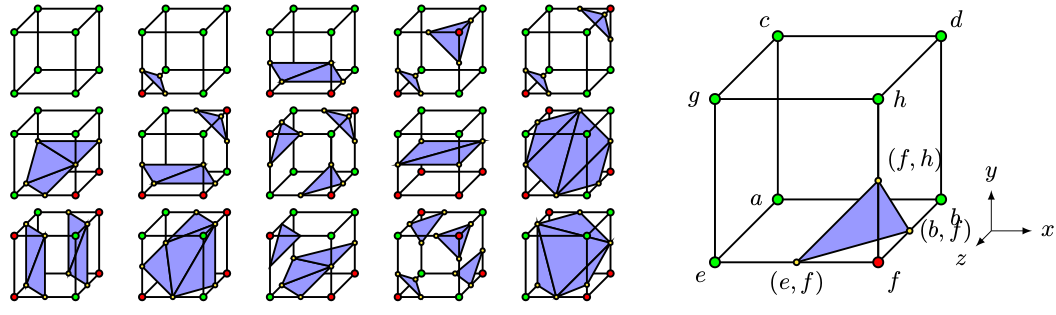
\includegraphics[width=\textwidth]{marching-cubes}
  \caption{Базовые предопределённые треугольники.}
  \label{fig:marching-cubes}
\end{figure}

Данный метод рассматривает все возможные комбинации точек со значением больше и со значением меньше заданного. С учетом симметрии в \cite{lorensen} предложено, что различных возможных базовых комбинаций всего 15 (рис.~\ref{fig:marching-cubes}), а всего комбинаций~--- 256. Таким образом, мы заранее знаем набор примитивов (в данном случае, треугольников) которые будут отображаться. Следовательно мы можем заранее просчитать эти примитивы, а также их атрибуты (нормали, цвета, и так далее).

Размер сетки является первым признаком улучшения качества и точности получаемой изоповерхности. Чем меньше выбирается шаг сетки, тем больше получается вокселей, тем более гладкой и точной получается результирующая изоповерхность, но тем медленнее она будет обрабатываться и рисоваться.

Понятно, что большой набор возможных комбинаций (256) ставит задачу продуманной работы с такими большими массивами данных без потери производительности и с достаточной степенью гибкости для возможности дальнейших оптимизаций. Рассмотрим основные оптимизации.

Для начала, основываясь на принятой нами индексации вершин, составляется идентификатор комбинации, который может принимать значение от 0 до 255 (по числу возможных вариантов). Так как каждая вершина может находится только в двух состояниях, то считается он следующим образом:
\begin{equation} \label{eq:case}
  I = \prod_{i=0}^{7} 2^i \cdot s(p_i, l), \quad s(x, y) =
  \begin{cases}
    1, & x \leq y \\
    0 & \text{иначе}
  \end{cases},
\end{equation}
\begin{conditions}
  $p_i$ & значение в вершине $i$;\\
  $l$ & заданный уровень изоповерхности.
\end{conditions}

Далее строится таблица, которая для каждого индекса, подсчитанного указанным выше способом, определяет те ребра, которые будет пересекать изоповерхность. Так как ребер всего 12, то данная таблица содержит 12-битные числа, подсчитанные аналогичным способом. Данную таблицу необходимо использовать для того, чтобы определить позицию вершины очередного треугольника.

Теперь, зная ребро, на которой будет находится вершина треугольника, вычислим её координаты. Как уже говорилось выше, позиция точки зависит от значений потенциала в вершинах и значения уровня изоповерхности:
\begin{equation} \label{eq:vertex}
  \vect v = \vect v_i + (l - p_i)\frac{\vect v_j - \vect v_i}{p_j - p_i},
\end{equation}
\begin{conditions}
  $i$ и $j$ & вершины, связанные ребром;\\
  $\vect v_i$ и $\vect v_j$ & координаты вершин $i$ и $j$.
\end{conditions}

Заметим, что если не проводить интерполяцию, а использовать за искомое значение, например, середину ребра, то все возможные треугольники могут быть просчитаны заранее, и, как следствие, могут быть просчитаны заранее нормали и другие атрибуты для них, следовательно мы избавляемся от большой работы, которую нам иначе бы пришлось выполнять в реальном времени. Однако, приходится мириться с потерей качества. Следовательно, в приложениях, где требуется высокая точность построения, как в данной работе, необходимо проводить интерполяцию, а в приложениях, где построение изоповерхности используется лишь как дополнительный элемент визуализации, достаточно грубого, но быстрого построения изоповерхности с полным предвычислением геометрии.


\subsection{Гистограммные пирамиды}
Каждый воксель может порождать до четырёх треугольников, что ведёт к большому расходу памяти, часто превышающего ограничения GPU. Дело усложняется тем, что во время рендеринга необходимо обойти все воксели, так как любой из них мог дать треугольники, что очень неэффективно.

Для решения данной проблемы используется подход гистопирамид, позволяя получить список активных вокселей (то есть порождающих треугольники) из сильно разреженной сетки вокселей \cite{ziegler}.

На первом шаге метода производится последовательная свертка матрицы рассматриваемых вокселей в четыре раза на каждой итерации, создавая квадродеревья для последующего обхода (рис.~\ref{fig:histopyramid-builder}). Также в результате свертки мы имеем количество активных вокселей.

\begin{figure}[h]
  \centering
  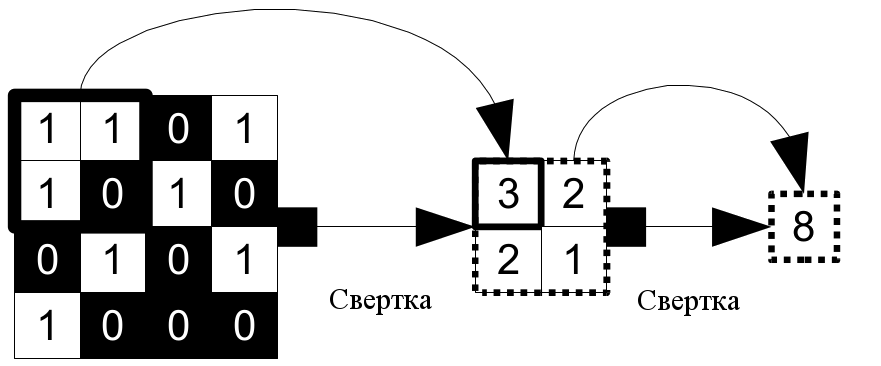
\includegraphics[width=.7\textwidth]{histopyramid-builder}
  \caption{Создание гистограммной пирамиды}
  \label{fig:histopyramid-builder}
\end{figure}

Следующим шагом создаётся непосредственно список активных вокселей. Для этого для каждого активного вокселя создаётся однозначное отображение индекса в координаты ячейки (рис.~\ref{fig:pointlist-builder}).

\begin{figure}[h]
  \centering
  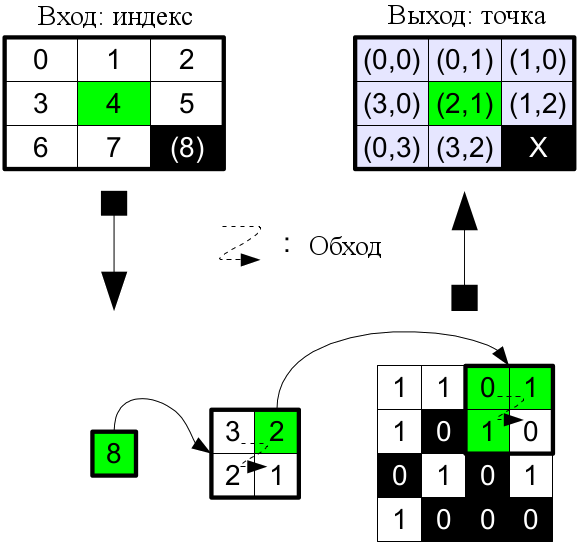
\includegraphics[width=.5\textwidth]{pointlist-builder}
  \caption{Создание списка активных вокселей}
  \label{fig:pointlist-builder}
\end{figure}

Стоит заметить, что порядок обхода неважен~--- главное, чтобы он был одинаков в обоих этапах.


\section{Рендеринг}
\subsection{Освещение}
Освещение в данной работе основано на использовании модели освещения Фонга \cite{phong}, полагая белый источника света. Метод требует сравнительно мало ресурсов, но большинство оптических явлений игнорируются либо рассчитываются с грубым приближением. В освещении по Фонгу интерполируется вектор нормали. Для нахождения вектора нормали в произвольной точке треугольника используют билинейную интерполяцию.

Рассмотрим следующие векторы (рис.~\ref{fig:lighting}):
\begin{itemize}
  \item $\uvect N$, нормаль к плоскости;
  \item $\uvect V$, направление к наблюдателю;
  \item $\uvect L$, направление к источнику света;
  \item $\uvect R$, отражённый луч источника света;
\end{itemize}

\begin{figure}[h]
  \centering
  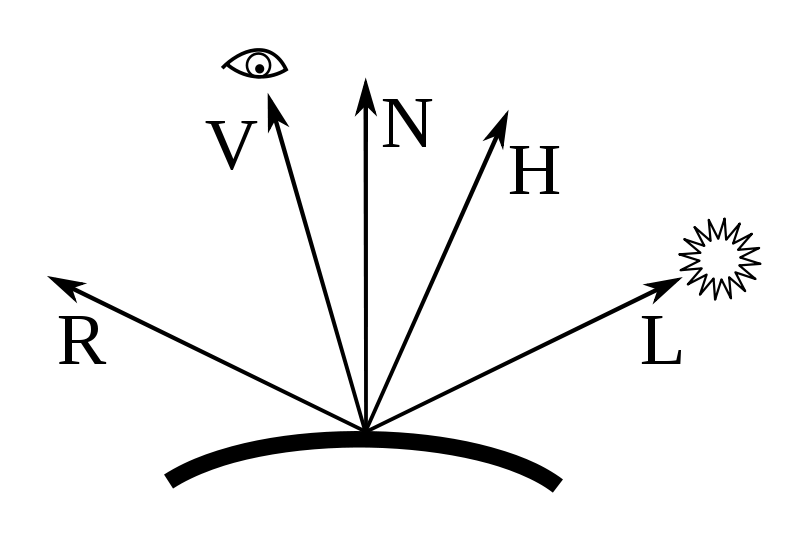
\includegraphics[width=.5\textwidth]{lighting}
  \caption{Векторы для вычисления освещения}
  \label{fig:lighting}
\end{figure}

В методе Фонга освещение раскладывается на три составляющие: фоновое, рассеянное и зеркальное освещение.

\subsubsection{Фоновое освещение}
Фоновое освещение~--- грубое приближение лучей света, рассеянных соседними объектами и затем достигших заданной точки:
\begin{equation} \label{eq:ambient}
  I_a=k_ac,
\end{equation}
\begin{conditions}
  $k_a$ & константа фонового освещения;\\
  $c$ & цвет поверхности в данной точке.
\end{conditions}

\subsubsection{Рассеянное освещение}
Рассеянное освещение~--- основная составляющая освещения:
\begin{equation} \label{eq:diffuse}
  I_d=k_d(\uvect L\cdot\uvect N)c,
\end{equation}
\begin{conditions}
  $k_d$ & константа рассеянного освещения;\\
  $c$ & цвет поверхности в данной точке.
\end{conditions}

\subsubsection{Зеркальное освещение}
Зеркальное освещение~--- составляющая освещения, отвечающая за зеркальность и матовость поверхности:
\begin{equation} \label{eq:specular}
  I_s=k_s(\uvect R\cdot\uvect V)^\alpha,
\end{equation}
\begin{conditions}
  $k_s$ & константа зеркального освещения;\\
  $\alpha$ & матовость поверхности.
\end{conditions}

Стоит заметить, что в уравнение не входит цвет поверхности, в отличие от других составляющих. Внешняя поверхность автомобиля является хорошим примером. Рассеянную составляющую обеспечивает краска, в то время как зеркальную~--- лак. Таким образом, часть лучей отражается, не доходя до краски.


\subsubsection{Затухание}
Затухание~--- эффект снижения интенсивности источника при его отдалении от поверхности. В реальном мире, интенсивность обратно пропорционально квадрату расстояния:
\[ I\propto\frac{1}{d^2}, \]
где $d$~--- расстояние от источника света до точки поверхности.

Однако для избежания возможного деления на нуль, будем использовать модифицированную версию:
\[ a=\frac{1}{1+d^2}, \]
где $a$ коэффициент затухания.

Во-вторых, для контроля над тем, как быстро интенсивность уменьшается с расстоянием, введём дополнительную константу:
\begin{equation} \label{eq:attenuation}
  a=\frac{1}{1+kd^2},
\end{equation}
\begin{conditions}
  $a$ & коэффициент затухания;\\
  $k$ & константа затухания.
\end{conditions}


\subsubsection{Итоговое уравнение}
Таким образом, итоговая формула принимает вид (рис.~\ref{fig:phong}):
\begin{equation} \label{eq:phong}
  I = k_ac + a\left(k_d(\uvect L\cdot\uvect N)c + k_s(\uvect R\cdot\uvect V)^\alpha\right),
\end{equation}
\[ a=\frac{1}{1+kd^2}, \]
\begin{conditions}
  $I$ & конечный цвет фрагмента;\\
  $c$ & цвет поверхности в данной точке;\\
  $k_a$ & константа фонового освещения;\\
  $k_d$ & константа рассеянного освещения;\\
  $k_s$ & константа зеркального освещения;\\
  $a$ & коэффициент затухания;\\
  $k$ & константа затухания;\\
  $d$ & расстояние от источника света до точки поверхности;\\
  $\uvect N$ & нормаль к плоскости;\\
  $\uvect V$ & направление к наблюдателю;\\
  $\uvect L$ & направление к источнику света;\\
  $\uvect R$ & отражённый луч источника света.
\end{conditions}

\begin{figure}[h]
  \centering
  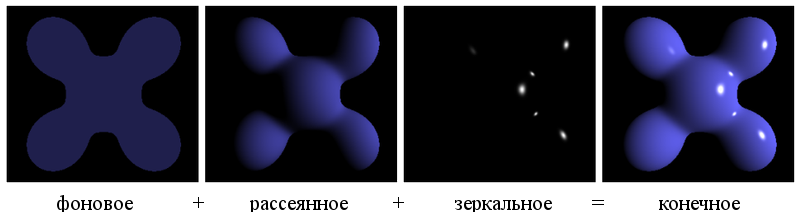
\includegraphics[width=\textwidth]{phong}
  \caption{Составляющие освещения.}
  \label{fig:phong}
\end{figure}


\subsection{Буфер глубины}
Буфер глубины представляет собой двумерный массив, каждый элемент которого соответствует пикселю на экране. Когда GPU рисует пиксель, его удалённость просчитывается и записывается в ячейку буфера глубины. Если пиксели двух рисуемых объектов перекрываются, то их значения глубины сравниваются, и рисуется тот, который ближе, а его значение удалённости сохраняется в буфер. По буферу глубины определяется удалённость от зрителя того или иного объекта трехмерной сцены.

Альтернативные алгоритмы (<<алгоритм художника>> и <<двоичное разбиение пространства>>) используются только при программной отрисовке, так как аппаратно эффективнее оказывается буфер глубины, поэтому в данной работе не рассматриваются.


\subsection{Полупрозрачность}
Полупрозрачность классически реализуется в два шага: в первую очередь рисуются все непрозрачные объекты с использованием буфера глубины, после чего рисуются полупрозрачные объекты в отсортированном по дальности порядке, причём буфер глубины используется, но не заполняется. При этом, если тест глубины пройден, то цвет получается смешиванием находящегося в буфере и обрабатываемого фрагмента цветов:
\begin{equation}
  o = s_as + (1-s_a)d \qquad o_a = s_a
\end{equation}
\begin{conditions}
  $s$ & значение цвета обрабатываемого фрагмента;\\
  $s_a$ & alpha-канал обрабатываемого фрагмента;\\
  $d$ & значение находящегося в буфере цвета;\\
  $o$ & значение результирующего цвета;\\
  $o_a$ & alpha-канал результата.
\end{conditions}

Стоит заметить, что в данной работе полупрозрачностью обладает только поверхность жидкости, а значит порядком отрисовки полупрозрачных объектов можно пренебречь.
